\documentclass[a4paper,11pt]{article}

\usepackage{textalpha}
\usepackage{multirow}
\usepackage{amsmath}
\usepackage{graphicx}
\usepackage{caption}

\title{1\textsuperscript{η} Υποχρεωτική Εργασία Στο Μάθημα της Αριθμητικής Ανάλυσης}

\author{Ονοματεπώνυμο: Βίκτωρ Κυρτσούδης \\ ΑΕΜ: 4143}

\date{}

\begin{document}

\maketitle

\begin{flushleft}
\boldmath

\section*{Άσκηση 1}
\begin{figure}[h]
    \caption*{Γραφική παράσταση των $f(x) = e^{sin^3x}+x^6-2x^4-x^3-1$ και \textbf{f'}}
    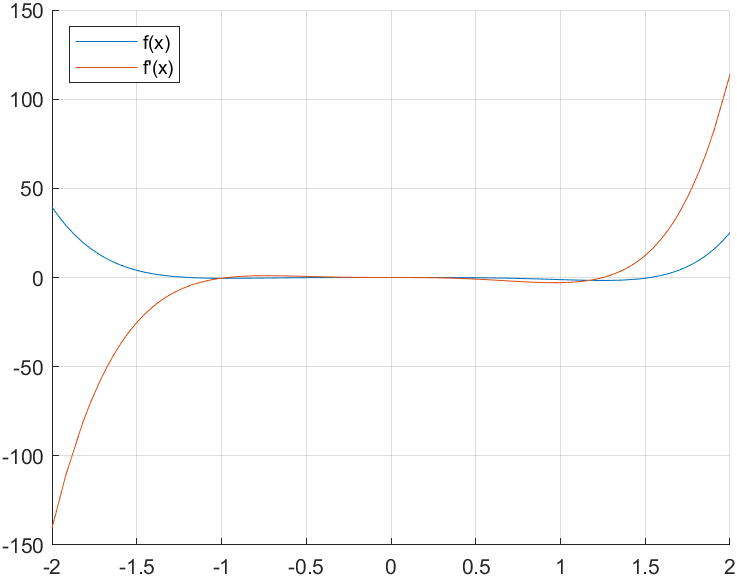
\includegraphics[width=\textwidth]{ex1plot.png}
\end{figure}

Από το γράφημα παρατηρούμε ότι:
\begin{enumerate}
    \item Η f φαίνεται να έχει ρίζες κοντά στα $x_1=-1$, $x_2=0$ και $x_3=1.5$.
    \item Η f' έχει ρίζα στο 0.
\end{enumerate}

Για τον υπολογισμό των ριζών δημιουργήθηκαν σε Matlab το πρόγραμμα ex1.m και οι συναρτήσεις bisection, newton και secant.

Στο ex1 ορίζεται μία συμβολική συνάρτηση f με τον αντίστοιχο τύπο, κατασκευάζεται το παραπάνω γράφημα και στην συνέχεια καλούνται με τη σειρά οι τρεις συναρτήσεις για να υπολογίσουν την κάθε ρίζα και των αριθμό των επαναλήψεων που χρειάζονται για να τις προσεγγίσουν. Τα αποτελέσματα για κάθε μέθοδο αποθηκεύονται στους πίνακες bisectionRoots, newtonRoots και secantRoots.
\linebreak

    
    
    \begin{table}[h]
        \centering
    \begin{tabular}{|c|c|c|c|}
        \hline
        \multirow{2}{*}{Μέθοδος} & -1.1976 & 0.0000 & 1.5301 \\ \cline{2-4}  & \multicolumn{3}{c|}{Επαναλήψεις} \\
        \hline
        Bisection & 18 & - & 18 \\ \hline
        Newton & 8 & 36 & 7 \\  \hline
        Secant & 14 & 55 & 10 \\ \hline
    \end{tabular}
\end{table}

\subsection*{Διχοτόμηση}
Η συνάρτηση bisection δέχεται την συνάρτηση $f$, το μέγιστο επιτρεπόμενο σφάλμα και τα ακρά του διαστήματος στο οποίο θα γίνει η αναζήτηση. Αφού υπολογίσει τον ελάχιστο αριθμο των αναγκαίων επαναλήψεων με τον τύπο 
$N > \frac{\ln{\frac{b-a}{\epsilon}}}{\ln{2}}$ 
ελέγχει αν το μέσο του διαστήματος είναι ρίζα της $f$ και αν ναι σταματάει και επιστρέφει τα αντίστοιχα αποτελέσματα. Αν δεν είναι αποφασίζει αν θα αντικαταστήσει το αριστερό ή το δεξί άκρο του διαστήματος με το μέσο δεδομένου ότι μετά την αντικατάσταση πρέπει να ισχύει: $f(a)*f(b)<0$. Και επαναλαμβάνει μέχρι να βρει την ρίζα ή να φτάσει τις $N$ Επαναλήψεις.
\linebreak

Χρησιμοποιούμε την μέθοδο της διχοτόμησης μόνο για την αναζήτηση των ριζών κοντά στο -1 και στο 1.5 γιατί κοντά στο 0 δεν υπάρχει διάστημα $[a,b]$ που να ισχύει $f(a)*f(b)<0$
\linebreak

\subsection*{Newton-Raphson}
Η συνάρτηση newton δέχεται την συνάρτηση $f$, το μέγιστο επιτρεπόμενο σφάλμα και το αρχικό σημείο $x_0$. Αρχικά υπολογίζει την νέα προσέγγιση με τον επαναληπτικό τύπο $x_{n+1} = x_n-\frac{f(x_n)}{f'(x_n)}$ και την διαφορά των προσεγγίσεων. Μετά ξεκινάει η επαναληπτική διαδικασία κατά την οποία ελέγχει αν η διαφορά είναι μεγαλύτερη του μέγιστου επιτρεπόμενου σφάλματος. Αν δεν είναι τερματίζει και επιστρέφει τα αποτελέσματα. Αν είναι υπολογίζει την νέα προσέγγιση και διαφορά. Αν η καινούρια διαφορά των τελευταίων προσεγγίσεων είναι μεγαλύτερη από την προηγούμενη τότε σημαίνει ότι δεν συγκλίνει οπότε σταματάει και επιστρέφει $NaN$ στην προσέγγιση και $0$ στις επαναλήψεις.
\linebreak

Παρόλο που στο 0 δεν υπάρχει διάστημα που να ικανοποιεί τις συνθήκες του θεωρήματος ύπαρξης μοναδικής ρίζας (δηλ. $f'(x),f''(x)\neq0$ για κάθε $x\in[a,b]$ και $f(a)*f(b)<0$) η Newton-Raphson επιστρέφει τα σωστά αποτελέσματα.
Επειδή όμως το 0 είναι ρίζα και της $f'$ (από το γράφημα) προκύπει ότι σε αντίθεση με τις ρίζες -1.1976 και 1.5301 δεν συγκλίνει τετραγωνικά στο 0 γι' αυτό και χρειάζονται τόσες παραπάνω επαναλήψεις.
\linebreak

\subsection*{Τέμνουσα}
Η συνάρτηση secant δέχεται την συνάρτηση $f$, το μέγιστο επιτρεπόμενο σφάλμα και τις αρχικές προσεγγίσεις $x_0$ και $x_1$. Μέχρι οι διαφορά των δύο τελευταίων προσεγγίσεων να γίνει μικρότερη του σφάλματος επαναλαμβάνει την εξής διαδικασία: υπολογίζει την νέα προσέγγιση με βάση τις προηγούμενες δύο χρησιμοποιώντας τον τύπο $x_{n+1} = x_n-\frac{f(x_n)(x_n-x_{n-1})}{f(x_n)-f(x_{n-1})}$ και μόλις γίνει αυτό επιστρέφει τα αποτελέσματα. 
\linebreak
Στο 0 ισχύει ό,τι ισχύει και στην Newton-Raphson.


\section*{Άσκηση 2}

\end{flushleft}
\end{document}